\def \typInto {Typesystem Introduction}
\section{Introduction}

\begin{frame}
  \frametitle{Are Typesystems Useful?}
  
  \begin{itemize}
    \item Advent of DSLs and DSL tools
    \item Writing languages easy, even for complex domains
    \item Complex languages $\Rightarrow$ complex constraint checking
    \item Most languages have a concept of \textbf{types}: reusable building
    blocks for constraints
  \end{itemize}
  
  \pause
  In this presentation:
  \begin{itemize}
    \item Using Xtext as DSL development environment
    \item Case study: form based editing of entities
    \item Compare different type system approaches
  \end{itemize}
\end{frame}

\begin{frame}
	\frametitle{\typInto} % for adjustments use overpic[grid,tics=10]  
	\begin{overpic}[scale=0.6]%
       {img/form-valid.png}
       \only<2>{
        \put(55,-40){\includegraphics[scale=0.6]%
		{img/form-invalid.png}}}
     \end{overpic}
\end{frame}

\begin{frame}[fragile]
  \frametitle{\typInto}
  \begin{columns}[T]
        \column{.6\textwidth}
        \begin{itemize}
    \item Static type checking example
        \end{itemize}
        % Generator: GNU source-highlight, by Lorenzo Bettini, http://www.gnu.org/software/src-highlite
\begin{tabular}[t]{l}
\noindent
\mbox{}name\ :\ \textbf{\textcolor{Plum}{string}}; \\
\mbox{}greeting\ =\ \textcolor{RoyalBlue}{"{}Hello\ "{}}\ +\ name\ +\ \textcolor{RoyalBlue}{"{}!"{}}; \\
\mbox{}
\end{tabular}

        \column{.4\textwidth}
        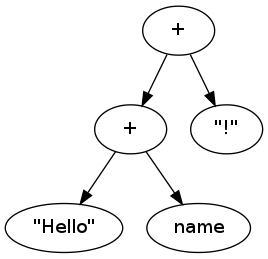
\includegraphics[scale=0.45]{img/ast1.png}
  \end{columns}
  \pause
  Common type system tasks:

  \begin{itemize}
    \item Assign fixed types to language elements
    \item Subtyping: is a type conformant to another type?
    \item Infer types of complex expressions
  \end{itemize}
\end{frame}